% 2018 全国Ⅰ卷 理18：正方形 ABCD 沿 DF 折起，C 到达 P（PF⊥BF）
% 底面为直角梯形 ABFD，E 为 AD 中点；虚线 C 为折叠前位置
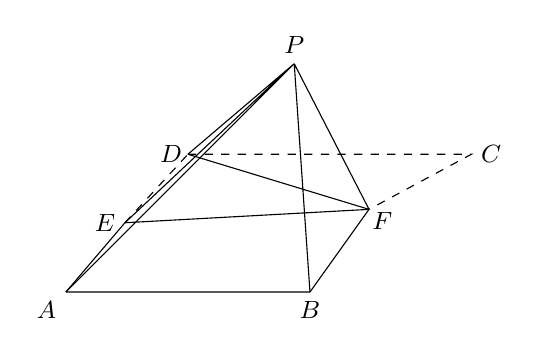
\begin{tikzpicture}[scale=1.0, font=\small]
  \coordinate (A) at (0,0);
  \coordinate (B) at (3.1,0);
  \coordinate (F) at (3.85,1.05);
  \coordinate (D) at (1.55,1.75);
  \coordinate (E) at (0.75,0.88);
  \coordinate (P) at (2.9,2.9);
  \coordinate (C) at (5.15,1.75);
  \draw (A) -- (B) -- (F);
  \draw (A) -- (E);
  \draw[dashed] (E) -- (D);
  \draw (D) -- (F);          % 折痕
  \draw (E) -- (F);
  \draw (A) -- (P)  (B) -- (P)  (F) -- (P)  (D) -- (P)  (E) -- (P);
  \draw[dashed] (D) -- (C) -- (F);
  \node[below left] at (A) {$A$};
  \node[below] at (B) {$B$};
  \node[below right, inner sep=1pt] at (F) {$F$};
  \node[left, inner sep=2pt] at (D) {$D$};
  \node[left] at (E) {$E$};
  \node[above] at (P) {$P$};
  \node[right] at (C) {$C$};
\end{tikzpicture}
